\documentclass[12pt]{article}

% Use packages %
\usepackage{graphicx, courier, amsmath, amssymb, amscd, amsfonts, mathtools, bm, esint, leftidx, extarrows, latexsym, relsize, color, tikz, comment, stmaryrd, float}
\usepackage[obeyspaces]{url}% http://ctan.org/pkg/url

% Set length %
\setlength{\textwidth}{160mm}
\setlength{\textheight}{235mm}
\setlength{\oddsidemargin}{-0mm}
\setlength{\topmargin}{-10mm}

% Define h-bar %
\newsavebox{\myhbar}
\savebox{\myhbar}{$\hbar$}
\renewcommand*{\hbar}{\mathalpha{\usebox{\myhbar}}}

% Chinese input %
%\usepackage{xeCJK} 
%\setCJKmainfont{微軟正黑體}
%\usepackage[T1]{fontenc}
%\makeatletter

% Equation number %
%\@addtoreset{equation}{section} 
%\renewcommand\theequation{{\thesection}.{\arabic{equation}}}
%\makeatletter 

% Helper Command %
\newcommand{\argmin}{\operatornamewithlimits{argmin}}
\newcommand{\rmnum}[1]{\romannumeral #1} 
\newcommand{\Rmnum}[1]{\expandafter\@slowromancap\romannumeral #1@}
\newcommand{\overbar}[1]{\mkern 1.5mu\overline{\mkern-1.5mu#1\mkern-1.5mu}\mkern 1.5mu}
\makeatother
\newcommand*{\QEDA}{\hfill\ensuremath{\blacksquare}}
\newcommand*{\QEDB}{\hfill\ensuremath{\square}}
\newcommand*{\BmVert}{\bigm\vert}
\newcommand{\bigslant}[2]{{\raisebox{.2em}{$#1$}\left/\raisebox{-.2em}{$#2$}\right.}}
\newcommand{\Nelements}[3]{\left\{ #1, ~ #2, \ldots, ~ #3 \right\}}
\newcommand{\CBrackets}[1]{\left\{#1\right\}}
\newcommand{\SBrackets}[1]{\left[#1\right]}
\newcommand{\BooBrackets}[1]{\left\llbracket#1\right\rrbracket}
\newcommand{\ParTh}[1]{\left(#1\right)}
\newcommand{\Ceil}[1]{\left\lceil#1\right\rceil}
\newcommand{\Floor}[1]{\left\lfloor#1\right\rfloor}
\newcommand{\BF}[1]{{\bf#1}}
\newcommand{\Inverse}[1]{{#1}^{-1}}
\newcommand{\Generator}[1]{\left\langle#1\right\rangle}
\newcommand{\AbsVal}[1]{\left|#1\right|}
\newcommand{\VecAbsVal}[1]{\left\|#1\right\|}
\newcommand{\BSlash}[2]{\left.#1\middle\backslash#2\right.}
\newcommand{\Divide}[2]{\left.#1\middle/#2\right.}
\newcommand{\SciNum}[2]{#1\times{10}^{#2}}
\newcommand{\Matrix}[2]{\ParTh{\begin{array}{#1}#2\end{array}}}
\newcommand{\MatrixTwo}[4]{\ParTh{\begin{array}{cc}{#1}&{#2}\\{#3}&{#4}\end{array}}}
\newcommand{\MatrixNByN}[1]{\Matrix{cccc}{{#1}_{11} & {#1}_{12} & \cdots & {#1}_{1n} \\ {#1}_{21} & {#1}_{22} & \cdots & {#1}_{2n} \\ \vdots & \vdots & \ddots & \vdots \\ {#1}_{n1} & {#1}_{n2} & \cdots & {#1}_{nn}}}
\newcommand{\ndiv}{\hspace{-4pt}\not|\hspace{2pt}}
\newcommand{\eqdef}{\xlongequal{\text{def}}}%
\newcount\arrowcount
\newcommand\arrows[1]{\global\arrowcount#1 \ifnum\arrowcount>0
\begin{matrix}\expandafter\nextarrow\fi}
\newcommand\nextarrow[1]{\global\advance\arrowcount-1 \ifx\relax#1\relax\else \xrightarrow{#1}\fi\ifnum\arrowcount=0 \end{matrix}\else\\\expandafter\nextarrow\fi}
\newcommand{\horrule}[1]{\rule{\linewidth}{#1}}

% Tikz settings %
\usetikzlibrary{shapes,arrows,positioning}
\tikzstyle{decision} = [diamond, draw, fill=white!20, text width=4.5em, text badly centered, node distance=3cm, inner sep=0pt]
\tikzstyle{block}    = [rectangle, draw, fill=white!20, text centered, rounded corners, minimum height=4em]
\tikzstyle{point}    = [fill = white!20, minimum size=0.5cm]
\tikzstyle{line}     = [draw, -latex']
\tikzstyle{mapsto}   = [draw, |->]
\tikzstyle{cloud}    = [draw, circle, minimum height=2em]

\begin{document}

\baselineskip 6.5mm
\setlength{\parindent}{0pt}
\title{ 
\normalfont \normalsize 
\horrule{0.5pt} \\[0.4cm]
\huge { \Huge Machine Learning \\ \large Answer Sheet for Homework 7}\\
\horrule{2pt} \\ [0.5cm]
}
\author{ { \Large Da-Min HUANG } \\
{\small R04942045} \\
{\small\textit{Graduate Institute of Communication Engineering, National Taiwan University}}
}
\date{January 6, 2016}
%\allowdisplaybreaks[4]
\maketitle

\subsection*{Problem 1}

Set $\mu_-=1-\mu_+$, we have
\begin{align}
1-\mu^2_+-\mu^2_-&=1-\mu^2_+-\ParTh{1-\mu_+}^2=\ParTh{1-\mu_+}\ParTh{1+\mu_+}-\ParTh{1-\mu_+}^2\\
&=2\mu_+\ParTh{1-\mu_+}=-2\mu^2_++2\mu_+=-2\ParTh{\mu_+-\dfrac{1}{2}}^2+\dfrac{1}{2}\\
&\leq\dfrac{1}{2}
\end{align}
Hence, if $\mu_+=\Divide{1}{2}\in\SBrackets{0,1}$, then the maximum value of Gini index is $\Divide{1}{2}$.

\QEDB

\horrule{0.5pt}

\subsection*{Problem 2}

The normalized Gini index is
\begin{align}
\dfrac{\ParTh{1-\mu^2_+-\mu^2_-}}{\ParTh{\dfrac{1}{2}}}=2\ParTh{1-\mu^2_+-\mu^2_-}
\end{align}
The squared error can be rewritten as
\begin{align}
\mu_+\ParTh{1-\ParTh{\mu_+-\mu_-}}^2+\mu_-\ParTh{-1-\ParTh{\mu_+-\mu_-}}^2&=4\mu_+\ParTh{1-\mu_+}^2+4\mu^2_+\ParTh{1-\mu_+}\\
&=4\mu_+\ParTh{1-\mu_+}\leq4\times\dfrac{1}{4}=1
\end{align}
Hence the normalized squared error is
\begin{align}
4\mu_+\ParTh{1-\mu_+}&=2\ParTh{2\mu_+\ParTh{1-\mu_+}}=2\ParTh{\ParTh{1-\mu_+}\ParTh{1+\mu_+}-\ParTh{1-\mu_+}^2}\\
&=2\ParTh{1-\mu^2_+-\mu^2_-}
\end{align}
which is equal to normalized Gini index.

\QEDB

\horrule{0.5pt}

\subsection*{Problem 3}

The probability of one example not sampled is
\begin{align}
\ParTh{1-\dfrac{1}{N}}^{pN}=\dfrac{1}{\ParTh{\dfrac{N}{N-1}}^{pN}}=\dfrac{1}{\ParTh{1+\dfrac{1}{N-1}}^{pN}}=\ParTh{\dfrac{1}{\ParTh{1+\dfrac{1}{N-1}}^{N}}}^p
\end{align}
As $N\rightarrow\infty$, we have
\begin{align}
\lim\limits_{N\rightarrow\infty}\ParTh{\dfrac{1}{\ParTh{1+\dfrac{1}{N-1}}^{N}}}^p=\ParTh{\lim\limits_{N\rightarrow\infty}\dfrac{1}{\ParTh{1+\dfrac{1}{N-1}}^{N}}}^p=\ParTh{\dfrac{1}{e}}^p=e^{-p}
\end{align}
So there approximately $e^{-p}\cdot N$ of the examples not sampled.

\QEDB

\horrule{0.5pt}

\subsection*{Problem 4}

Since $G=\text{Uniform}\ParTh{\CBrackets{g_k}^3_{k=1}}$, so if at least two terms of $\CBrackets{g_k}^3_{k=1}$ ouput wrong result, then $G$ outputs wrong result. Let $\CBrackets{E_k}^3_{k=1}$ be the set of examples that $\CBrackets{g_k}^K_{k=1}$ got wrong results. Apparently $\AbsVal{E_3}>\AbsVal{E_2}>\AbsVal{E_1}$ and $\AbsVal{E_1}+\AbsVal{E_2}>\AbsVal{E_3}$. So
\begin{enumerate}
	\item Maximum of $E_{\text{out}}\ParTh{G}$ happens at $E_3\subset\ParTh{E_1\cup E_2}$. Then $G$ outputs wrong result in the region of $E_3$ with $E_{\text{out}}\ParTh{G}=0.35$.
	\item Minimum of $E_{\text{out}}\ParTh{G}$ happens at $E_i\cap E_j=\phi$, $i\neq j$ and $1\leq i,j\leq 3$ with $i,j\in\mathbb{N}$. Then $G$ always ouputs the correct result since $\ParTh{E_1\cup E_2\cup E_3}\subset\CBrackets{\text{all examples}}$.
\end{enumerate}
Hence, $0\leq E_{\text{out}}\ParTh{G}\leq0.35$.
\begin{comment}
\begin{align}
\nonumber
&~0.15\times0.25\times0.65+0.25\times0.35\times0.85+0.15\times0.35\times0.75+0.15\times0.25\times0.35\\
=&~0.15125
\end{align}
\end{comment}

\QEDB

\horrule{0.5pt}

\subsection*{Problem 5}

Since $G=\text{Uniform}\ParTh{\CBrackets{g_k}^K_{k=1}}$, so if at least $\Divide{\ParTh{K+1}}{2}$ terms of $\CBrackets{g_k}^K_{k=1}$ ouput wrong result, then $G$ outputs wrong result. Let $\CBrackets{E_k}^K_{k=1}$ be the set of examples that $\CBrackets{g_k}^K_{k=1}$ got wrong results.

If $G$ outputs wrong result on some example $\BF{x}$, then we have
\begin{align}
\BF{x}\in\bigcap^{\ParTh{\frac{{K+1}}{2}}+m}_{i=1}E_{\alpha_i}
\end{align}
where $\alpha_i\in\CBrackets{1,2,\ldots,K}$ satisfies $1\leq\alpha_i\leq K$ and $m\in\ParTh{\mathbb{N}\cup\CBrackets{0}}$ with $0\leq m<\Divide{{K+1}}{2}$. And
\begin{align}
\AbsVal{\bigcap^{\ParTh{\frac{{K+1}}{2}}+m}_{i=1}E_{\alpha_i}}\leq\dfrac{2}{K+1+2m}\sum_{k=1}^{K}e_k\leq\dfrac{2}{K+1}\sum_{k=1}^{K}e_k
\label{5-1}
\end{align}
(\ref{5-1}) holds due to %$\AbsVal{\bigcap^{\ParTh{\Divide{\ParTh{K+1}}{2}}+m}_{i=1}E_{\alpha_i}}\leq\frac{2}{K+1+2m}\sum_{k=1}^{K}e_k$ holds due to
\begin{align}
\bigcap^{\ParTh{\frac{{K+1}}{2}}+m}_{i=1}E_{\alpha_i}\subseteq E_{\beta}\text{ with }\AbsVal{E_\beta}\leq\AbsVal{E_{\alpha_i}},~\forall i
\end{align}
where $\beta$ is some index such that $\AbsVal{E_{\beta}}=\min_{\alpha_i}\AbsVal{E_{\alpha_i}}$. So
\begin{align}
\ParTh{\dfrac{K+1}{2}+m}\AbsVal{\bigcap^{\ParTh{\frac{{K+1}}{2}}+m}_{i=1}E_{\alpha_i}}&\leq\ParTh{\dfrac{K+1}{2}+m}\AbsVal{E_{\beta}}\leq\sum_{i=1}^{\ParTh{\frac{{K+1}}{2}}+m}\AbsVal{E_{\alpha_i}}\leq\sum_{k=1}^{K}\AbsVal{E_k}
\label{5-2}
\end{align}
(\ref{5-2}) holds since size of $E_\beta$ is the samllest among $\ParTh{\ParTh{\frac{{K+1}}{2}}+m}$ terms and $\sum_{k=1}^{K}\AbsVal{E_k}$ must contains the $\ParTh{\ParTh{\frac{{K+1}}{2}}+m}$ terms. Hence, we have
\begin{align}
E_{\text{out}}\ParTh{G}\leq\dfrac{2}{K+1+2m}\sum_{k=1}^{K}e_k\leq\dfrac{2}{K+1}\sum_{k=1}^{K}e_k
\end{align}
where $\AbsVal{E_k}=e_k$ by definition.
\begin{comment}
\begin{align}
\dfrac{2}{M+1}\sum_{k=1}^{M}e_k\leq\dfrac{2}{M+3}\sum_{k=1}^{M+2}e_k=\dfrac{2}{M+3}\ParTh{\sum_{k=1}^{M}e_k+e_{M+1}+e_{M+2}}
\end{align}
\begin{align}
\dfrac{4}{\ParTh{M+1}\ParTh{M+3}}\sum_{k=1}^{M}e_k-e_{M+1}-e_{M+2}
\end{align}
\end{comment}

\QEDB

\horrule{0.5pt}

\subsection*{Problem 6}

By the definition of $U_{t}$, we have
\begin{align}
U_{t+1}&=\dfrac{1}{N}\sum_{n=1}^{N}\exp\ParTh{-y_n\sum_{\tau=1}^{t}\alpha_\tau g_\tau\ParTh{\BF{x}_n}}\\
&=\dfrac{1}{N}\sum_{n=1}^{N}\exp\ParTh{-y_n\sum_{\tau=1}^{t-1}\alpha_\tau g_\tau\ParTh{\BF{x}_n}-y_n\alpha_tg_t\ParTh{\BF{x}_n}}\\
&=\dfrac{1}{N}\sum_{n=1}^{N}\exp\ParTh{-y_n\sum_{\tau=1}^{t-1}\alpha_\tau g_\tau\ParTh{\BF{x}_n}}\exp\ParTh{-y_n\alpha_tg_t\ParTh{\BF{x}_n}}\\%=U_{t}\exp\ParTh{\alpha_tg_t\ParTh{\BF{x}_n}}\\
&=\sum_{n=1}^{N}u^{\ParTh{t}}_n\exp\ParTh{-y_n\alpha_tg_t\ParTh{\BF{x}_n}}\\
&=\sum_{\substack{n \\ y_n\neq g_t\ParTh{\BF{x}_n}}}u^{\ParTh{t}}_n\exp\ParTh{-y_n\alpha_tg_t\ParTh{\BF{x}_n}}+\sum_{\substack{n \\ y_n=g_t\ParTh{\BF{x}_n}}}u^{\ParTh{t}}_n\exp\ParTh{-y_n\alpha_tg_t\ParTh{\BF{x}_n}}\\
&=\sum_{\substack{n \\ y_n\neq g_t\ParTh{\BF{x}_n}}}u^{\ParTh{t}}_n\exp\ParTh{\alpha_t}+\sum_{\substack{n \\ y_n=g_t\ParTh{\BF{x}_n}}}u^{\ParTh{t}}_n\exp\ParTh{-\alpha_t}\\
&=\exp\ParTh{\alpha_t}\ParTh{\epsilon_t}\sum_{n=1}^{N}u^{\ParTh{t}}_n+\exp\ParTh{-\alpha_t}\ParTh{1-\epsilon_t}\sum_{n=1}^{N}u^{\ParTh{t}}_n\\
&=U_t\ParTh{\exp\ParTh{\alpha_t}\ParTh{\epsilon_t}+\exp\ParTh{-\alpha_t}\ParTh{1-\epsilon_t}}=U_t\cdot2\sqrt{\epsilon_t\ParTh{1-\epsilon_t}}
\end{align}
Since
\begin{align}
U_{1}=\sum_{n=1}^{N}u^{\ParTh{1}}_n=\sum_{n=1}^{N}\dfrac{1}{N}=1
\end{align}
we have
\begin{align}
U_3&=U_2\cdot2\sqrt{\epsilon_2\ParTh{1-\epsilon_2}}=\ParTh{U_1\cdot2\sqrt{\epsilon_1\ParTh{1-\epsilon_1}}}\cdot2\sqrt{\epsilon_2\ParTh{1-\epsilon_2}}\\
&=4\sqrt{\epsilon_1\epsilon_2\ParTh{1-\epsilon_1}\ParTh{1-\epsilon_2}}
\end{align}
which can be generalized as
\begin{align}
U_{T+1}=\prod_{t=1}^{T}\ParTh{2\sqrt{\epsilon_t\ParTh{1-\epsilon_t}}}
\end{align}

\QEDB

\horrule{0.5pt}

\subsection*{Problem 7}

To compute $s_n$, we need to find the optimal $\eta$ of
\begin{align}
\min_\eta\dfrac{1}{N}\sum_{n=1}^{N}\ParTh{\ParTh{y_n-s_n}-\eta g_t\ParTh{\BF{x}_n}}^2\coloneqq A
\end{align}
From $\Divide{\partial A}{\partial\eta}=0$, we have
\begin{align}
\eta=\dfrac{\sum_{n=1}^{N}g_t\ParTh{\BF{x}_n}\ParTh{y_n-s_n}}{\sum_{n=1}^{N}g^2_t\ParTh{\BF{x}_n}}
\end{align}
Now $s_n=0$ and $g_1\ParTh{\BF{x}}=2$, so
\begin{align}
\eta=\dfrac{2\sum_{n=1}^{N}y_n}{4\sum_{n=1}^{N}}=\dfrac{1}{2N}\sum_{n=1}^{N}y_n
\end{align}
Since $\eta=\alpha_1$, so
\begin{align}
\alpha_1g_1\ParTh{\BF{x}_n}=\dfrac{2}{2N}\sum_{n=1}^{N}y_n=\dfrac{1}{N}\sum_{n=1}^{N}y_n=s_n
\end{align}

\QEDB

\horrule{0.5pt}

\subsection*{Problem 8}

From the equatio of optimal $\eta$, we have
\begin{align}
\eta=\dfrac{\sum_{n=1}^{N}g_t\ParTh{\BF{x}_n}\ParTh{y_n-s^\prime_n}}{\sum_{n=1}^{N}g^2_t\ParTh{\BF{x}_n}}=\dfrac{\sum_{n=1}^{N}y_ng_t\ParTh{\BF{x}_n}-\sum_{n=1}^{N}s^\prime_ng_t\ParTh{\BF{x}_n}}{\sum_{n=1}^{N}g^2_t\ParTh{\BF{x}_n}}=\alpha_t
\end{align}
so
\begin{align}
\sum_{n=1}^{N}y_ng_t\ParTh{\BF{x}_n}-\sum_{n=1}^{N}s^\prime_ng_t\ParTh{\BF{x}_n}=\alpha_t\sum_{n=1}^{N}g^2_t\ParTh{\BF{x}_n}=\sum_{n=1}^{N}\alpha_tg^2_t\ParTh{\BF{x}_n}=\sum_{n=1}^{N}\ParTh{s_n-s^\prime_n}g_t\ParTh{\BF{x}_n}
\end{align}
where $s^\prime_n$ is defined as the $s_n$ in iteration $\ParTh{t-1}$ and $s_n=s^\prime_n+\alpha_tg_t\ParTh{\BF{x}_n}$, so
\begin{align}
\sum_{n=1}^{N}s_ng_t\ParTh{\BF{x}_n}=\sum_{n=1}^{N}y_ng_t\ParTh{\BF{x}_n}
\end{align}
%Since all $s_n$ are updated in iteration $t$, we have

\QEDB

\horrule{0.5pt}

\subsection*{Problem 9}

$\text{OR}\ParTh{x_1,x_2,\ldots,x_d}$ means outputs TRUE if one input is TRUE; outputs FALSE if all inputs are FALSE.

\underline{Claim}: $\ParTh{w_0,w_1,\ldots,w_d}=\ParTh{d-1,1,\ldots,1}$ implements $\text{OR}$.

\underline{Proof of Claim}:
\begin{enumerate}
	\item If all $x_i=-1$, then we have
	\begin{align}
	\text{sign}\ParTh{\sum_{i=0}^{d}w_ix_i}=\text{sign}\ParTh{d-1+\sum_{i=1}^{d}\ParTh{-1}}=\text{sign}\ParTh{-1}=\text{FALSE}
	\end{align}
	\item If some $x_i=+1$ and others are $-1$, we have
	\begin{align}
	\text{sign}\ParTh{\sum_{i=0}^{d}w_ix_i}=\text{sign}\ParTh{d-1+1+\ParTh{-1}\ParTh{d-1}}=\text{sign}\ParTh{+1}=\text{TRUE}
	\end{align}
\end{enumerate}
Hence, $\ParTh{w_0,w_1,\ldots,w_d}=\ParTh{d-1,1,\ldots,1}$ implements $\text{OR}$.

\QEDB

\horrule{0.5pt}

\subsection*{Problem 10}

\underline{Claim}: $D\geq5$.

\underline{Proof of Claim}:

The weights of hidden layer and output layer are
\begin{align}
\text{Neuron 1}:&\ParTh{w^{\ParTh{1}}_{01},w^{\ParTh{1}}_{11},w^{\ParTh{1}}_{21},w^{\ParTh{1}}_{31},w^{\ParTh{1}}_{41},w^{\ParTh{1}}_{51}}=\ParTh{4,1,1,1,1,1}\\
\text{Neuron 2}:&\ParTh{w^{\ParTh{1}}_{02},w^{\ParTh{1}}_{12},w^{\ParTh{1}}_{22},w^{\ParTh{1}}_{32},w^{\ParTh{1}}_{42},w^{\ParTh{1}}_{52}}=\ParTh{2,1,1,1,1,1}\\
\text{Neuron 3}:&\ParTh{w^{\ParTh{1}}_{03},w^{\ParTh{1}}_{13},w^{\ParTh{1}}_{23},w^{\ParTh{1}}_{33},w^{\ParTh{1}}_{43},w^{\ParTh{1}}_{53}}=\ParTh{0,1,1,1,1,1}\\
\text{Neuron 4}:&\ParTh{w^{\ParTh{1}}_{04},w^{\ParTh{1}}_{14},w^{\ParTh{1}}_{24},w^{\ParTh{1}}_{34},w^{\ParTh{1}}_{44},w^{\ParTh{1}}_{54}}=\ParTh{-2,1,1,1,1,1}\\
\text{Neuron 5}:&\ParTh{w^{\ParTh{1}}_{05},w^{\ParTh{1}}_{15},w^{\ParTh{1}}_{25},w^{\ParTh{1}}_{35},w^{\ParTh{1}}_{45},w^{\ParTh{1}}_{55}}=\ParTh{-4,1,1,1,1,1}\\
\text{Output Neuron}:&\ParTh{w^{\ParTh{2}}_{01},w^{\ParTh{2}}_{11},w^{\ParTh{2}}_{21},w^{\ParTh{2}}_{31},w^{\ParTh{2}}_{41},w^{\ParTh{2}}_{51}}=\ParTh{\Divide{1}{5},1,-1,1,-1,1}
\end{align}
The values table is
\renewcommand\arraystretch{1.5}
\begin{center}
\begin{tabular}{ | c | c | c | }
  \hline
  Number of 1 in Inputs & Hidden Layer Output & Output \\ \hline
  0&$\ParTh{-1,-1,-1,-1,-1}$&-1 \\ \hline
  1&$\ParTh{+1,-1,-1,-1,-1}$&+1 \\ \hline
  2&$\ParTh{+1,+1,-1,-1,-1}$&-1 \\ \hline
  3&$\ParTh{+1,+1,+1,-1,-1}$&+1 \\ \hline
  4&$\ParTh{+1,+1,+1,+1,-1}$&-1 \\ \hline
  5&$\ParTh{+1,+1,+1,+1,+1}$&+1 \\ \hline
\end{tabular}
\end{center}
The condition of $D=5$ is the smallest choice left to be proven in Problem 21.

%From the conclusion of Problem 21, we have $D=5$.
\begin{comment}
\begin{enumerate}
	\item $D=5$ can implement $\text{XOR}$.
	
	We have
	\begin{align}
	\text{XOR}\ParTh{g_1,g_2}=\text{OR}\ParTh{\text{AND}\ParTh{-g_1,g_2},\text{AND}\ParTh{g_1,-g_2}}
	\end{align}
	Since there are 5 neurons in first layer, so we have $g_1,g_2,g_3$ and $g_4$ output to second layer. And
	\begin{align}
	\text{XOR}\ParTh{g_1,g_2,g_3,g_4}&=\text{XOR}\ParTh{\text{XOR}\ParTh{g_1,g_2},g_3,g_4}\\
	&=\text{XOR}\ParTh{\text{XOR}\ParTh{\text{XOR}\ParTh{g_1,g_2},g_3},g_4}
	\end{align}
	Use logistic operator to rewrite the equation, we have
	\begin{align}
	\text{XOR}\ParTh{\text{XOR}\ParTh{g_1,g_2},g_3}=g^{\prime}_1g^{\prime}_2g_3+g^{\prime}_1g_2g^{\prime}_3+g_1g^{\prime}_2g^{\prime}_3+g_1g_2g_3
	\end{align}
\end{enumerate}
\end{comment}

\QEDB

\horrule{0.5pt}

\subsection*{Problem 11}

\underline{Claim}: Only the gradient components with respect to $w^{\ParTh{L}}_{01}$ may be non-zero, all other gradient components must be zero.

\underline{Proof of Claim}:

Consider
\begin{align}
\dfrac{\partial e_n}{\partial w^{\ParTh{L}}_{i1}}=-2\ParTh{y_n-s^{\ParTh{L}}_1}\ParTh{x^{\ParTh{L-1}}_i}=-2\ParTh{y_n-\sum_{j=0}^{d^{\ParTh{L-1}}}w^{\ParTh{L}}_{j1}x^{\ParTh{L-1}}_j}\ParTh{x^{\ParTh{L-1}}_i}
\end{align}
Since all $w^{\ParTh{\ell}}_{ij}=0$, we have
\begin{align}
\dfrac{\partial e_n}{\partial w^{\ParTh{L}}_{i1}}=-2y_nx^{\ParTh{L-1}}_i%=-2y_n\tanh\ParTh{s^{\ParTh{L-1}}_i}=-2y_n\tanh\ParTh{\sum_{j=0}^{d^{\ParTh{L-1}}}w^{\ParTh{L-1}}_{ji}x^{\ParTh{L-2}}_j}
\end{align}
If $i\neq0$, then
\begin{align}
\dfrac{\partial e_n}{\partial w^{\ParTh{L}}_{i1}}=-2y_nx^{\ParTh{L-1}}_i=-2y_n\tanh\ParTh{s^{\ParTh{L-1}}_i}=-2y_n\tanh\ParTh{\sum_{j=0}^{d^{\ParTh{L-2}}}w^{\ParTh{L-1}}_{ji}x^{\ParTh{L-2}}_j}=0
\end{align}
since all $w^{\ParTh{\ell}}_{ij}=0$.

If $i=0$, then
\begin{align}
\dfrac{\partial e_n}{\partial w^{\ParTh{L}}_{01}}=-2y_nx^{\ParTh{L-1}}_0=-2y_n
\end{align}
If $y_n\neq0$, then
\begin{align}
\dfrac{\partial e_n}{\partial w^{\ParTh{L}}_{01}}\neq0
\end{align}
Similarly, we have
\begin{align}
\dfrac{\partial e_n}{\partial w^{\ParTh{\ell}}_{0j}}=\delta^{\ParTh{\ell}}_j\ParTh{x^{\ParTh{\ell-1}}_0}=\delta^{\ParTh{\ell}}_j=\sum_{k}\ParTh{\delta^{\ParTh{\ell+1}}_k}\ParTh{w^{\ParTh{\ell+1}}_{jk}}\ParTh{\dfrac{\partial\tanh\ParTh{s^{\ParTh{\ell}}_j}}{\partial s^{\ParTh{\ell}}_j}}=0
\end{align}
since all $w^{\ParTh{\ell}}_{ij}=0$.

\QEDB

\horrule{0.5pt}

\subsection*{Problem 12}

For $\ell=1$ and all $w^{\ParTh{\ell}}_{ij}$ initialized as 1, we have
\begin{align}
\eta x^{\ParTh{0}}_i\delta^{\ParTh{1}}_j&=\eta x^{\ParTh{0}}_i\sum_{k}\ParTh{\delta^{\ParTh{2}}_k}\ParTh{w^{\ParTh{2}}_{jk}}\ParTh{\dfrac{\partial\tanh\ParTh{s^{\ParTh{1}}_j}}{\partial s^{\ParTh{1}}_j}}\\
&=\eta x^{\ParTh{0}}_i\sum_{k}\ParTh{\delta^{\ParTh{2}}_k}\ParTh{\dfrac{\partial\tanh\ParTh{s^{\ParTh{1}}_j}}{\partial s^{\ParTh{1}}_j}}
\end{align}
and
\begin{align}
s^{\ParTh{1}}_j=\sum_{i=0}^{d^{\ParTh{0}}}w^{\ParTh{1}}_{ij}x^{\ParTh{0}}_i=\sum_{i=0}^{d^{\ParTh{0}}}x^{\ParTh{0}}_i
\end{align}
So we have
\begin{align}
s^{\ParTh{1}}_1=s^{\ParTh{1}}_2=\cdots=s^{\ParTh{1}}_{d^{\ParTh{1}}}\Rightarrow\delta^{\ParTh{1}}_1=\delta^{\ParTh{1}}_2=\cdots=\delta^{\ParTh{1}}_{d^{\ParTh{1}}}
\end{align}
Hence, all update term of $w^{\ParTh{1}}_{ij}$ is the same for $1\leq j\leq d^{\ParTh{1}}$, so
\begin{align}
w^{\ParTh{1}}_{ij}=w^{\ParTh{1}}_{i\ParTh{j+1}}
\end{align}
for $1\leq j\leq d^{\ParTh{1}}-1$.

\QEDB

\horrule{0.5pt}

\subsection*{Problem 13}

The rules of following tree are
\begin{enumerate}
	\item $\ParTh{\text{feature column},\text{ }s,\text{ }\theta}$. The meaning of combination of numbers.
	\item If the feature of $\BF{x}$ is smaller than $\theta$, then go to the left tree; if not, then go to the right tree.
	\item If go to left and there is no more node, then return $s\times\ParTh{+1}$; if go to the right and there is no more node, return $s\times\ParTh{-1}$, where $s$ is from the last node.
\end{enumerate}
\begin{comment}
root (1, 1.0, 0.62623300000000004)
	left  (0, -1.0, 0.22443950000000001)
		left  (1, 1.0, 0.11515275)
		right (0, -1.0, 0.54150799999999999)
			left  (1, 1.0, 0.35862050000000001)
				left  (0, 1.0, 0.50162499999999999)
				right (0, 1.0, 0.26075150000000002)
			right (1, -1.0, 0.28592499999999998)
				left  (1, 1.0, 0.26603850000000001)
	right (0, -1.0, 0.87817149999999999)
\end{comment}
\begin{figure}[H]
	\centering
	\begin{tikzpicture}[node distance = 3cm, auto]
	
		% Node Setting %
		
		% 0 =======================================%
		\node [block] (root) {$(1, 1.0, 0.626)$};
		% 1 =======================================%
		\node [block, below left of = root] (1st) {$(0, -1.0, 0.224)$};
		% 2 =======================================%
		\node [block, below left of = 1st] (3rd) {$(1, 1.0, 0.115)$};
		% 3 =======================================%
		\node [cloud, below left of = 3rd, yshift=0.5cm] (3rdL) {$+1$};
		\node [cloud, below of = 3rd, yshift=1.0cm] (3rdR) {$-1$};
		%=========================================%
		\node [block, below right of = 1st, xshift=-0.5cm] (4th) {$(0, -1.0, 0.542)$};
		% 3 =======================================%
		\node [block, below left of = 4th, xshift=0.5cm] (5th) {$(1, 1.0, 0.359)$};
		% 4 =======================================%
		\node [block, below left of = 5th, xshift=0.5cm] (7th) {$(0, 1.0, 0.502)$};
		% 5 =======================================%
		\node [cloud, below left of = 7th, yshift=0.5cm] (7thL) {$+1$};
		\node [cloud, below of = 7th, xshift=0.5cm, yshift=1.0cm] (7thR) {$-1$};
		%=========================================%
		\node [block, below right of = 5th, xshift=-0.6cm] (8th) {$(0, 1.0, 0.261)$};
		% 5 =======================================%
		\node [cloud, below left of = 8th, xshift=0.7cm, yshift=0.5cm] (8thL) {$+1$};
		\node [cloud, below right of = 8th, xshift=-1.0cm, yshift=0.5cm] (8thR) {$-1$};
		%=========================================%
		% 3 =======================================%
		\node [block, below right of = 4th, xshift=1.5cm] (6th) {$(1, -1.0, 0.286)$};
		% 4 =======================================%
		\node [block, below of = 6th, xshift=-0.8cm, yshift=1.0cm] (9th) {$(1, 1.0, 0.266)$};
		% 5 =======================================%
		\node [cloud, below of = 9th, xshift=-0.5cm, yshift=1.0cm] (9thL) {$+1$};
		\node [cloud, below right of = 9th, yshift=0.5cm] (9thR) {$-1$};
		%=========================================%
		\node [cloud, below right of = 6th, xshift=-0.5cm, yshift=0.5cm] (6thR) {$+1$};
		%=========================================%
		% 1 =======================================%
		\node [block, below right of = root] (2nd) {$(0, -1.0, 0.878)$};
		% 2 =======================================%
		\node [cloud, below of = 2nd, xshift=-0.2cm, yshift=1.0cm] (2ndL) {$-1$};
		\node [cloud, below right of = 2nd, yshift=0.5cm] (2ndR) {$+1$};
		%=========================================%
		
		% Connection %
		
		\path [line] (root)  -- (1st);
		\path [line] (1st)  -- (3rd);
		\path [line] (3rd)  -- (3rdL);
		\path [line] (3rd)  -- (3rdR);
		\path [line] (1st)  -- (4th);
		\path [line] (4th)  -- (5th);
		\path [line] (5th)  -- (7th);
		\path [line] (7th)  -- (7thL);
		\path [line] (7th)  -- (7thR);
		\path [line] (5th)  -- (8th);
		\path [line] (8th)  -- (8thL);
		\path [line] (8th)  -- (8thR);
		\path [line] (4th)  -- (6th);
		\path [line] (6th)  -- (9th);
		\path [line] (9th)  -- (9thL);
		\path [line] (9th)  -- (9thR);
		\path [line] (6th)  -- (6thR);
		\path [line] (root)  -- (2nd);
		\path [line] (2nd)  -- (2ndL);
		\path [line] (2nd)  -- (2ndR);
	\end{tikzpicture}
	\caption{Tree Graph} 
	\label{Tree}
\end{figure}

\QEDB

\horrule{0.5pt}

\subsection*{Problem 14}

$E_{\text{in}}=0.0$.

\QEDB

\horrule{0.5pt}

\subsection*{Problem 15}

$E_{\text{out}}=0.126$.

\QEDB

\horrule{0.5pt}

\subsection*{Problem 16}

\begin{figure}[H]
	\centering
	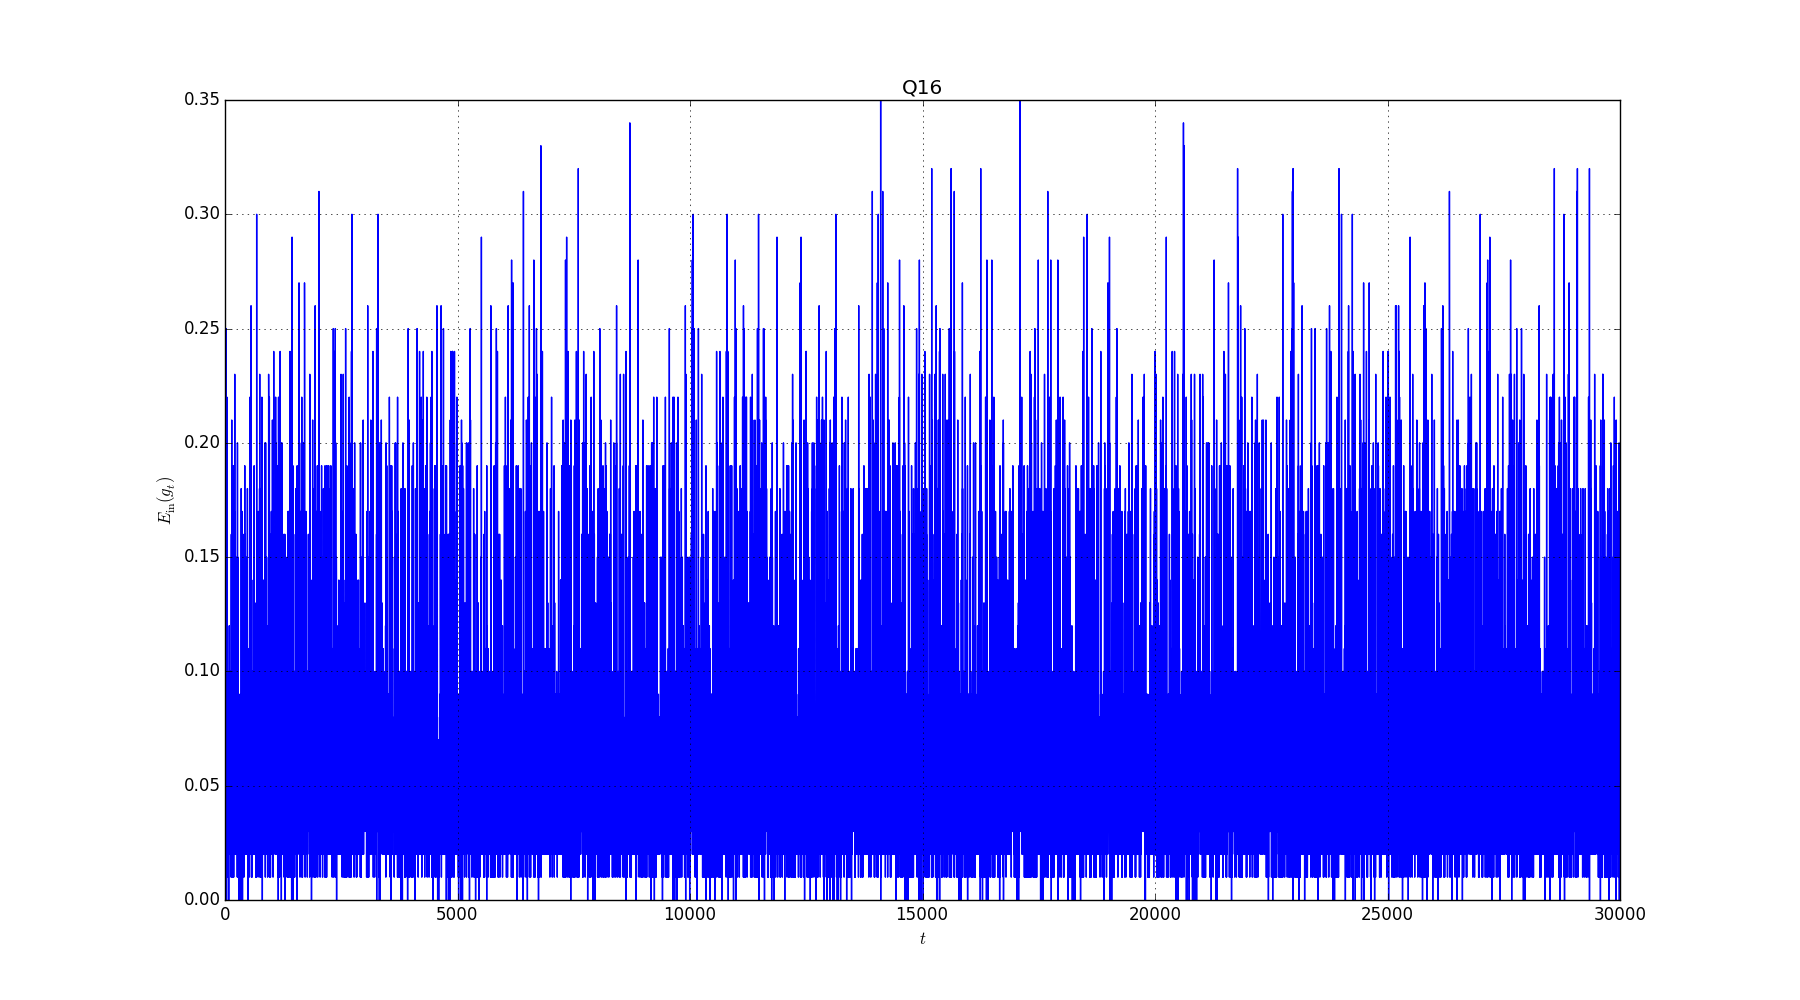
\includegraphics[scale=0.5]{Q16.png}
	\caption{Q16}
	\label{Q16}
\end{figure}
The average $E_{\text{in}}\ParTh{g_t}$ of total 30,000 trees is $0.0593$.

\QEDB

\horrule{0.5pt}

\subsection*{Problem 17}

\begin{figure}[H]
	\centering
	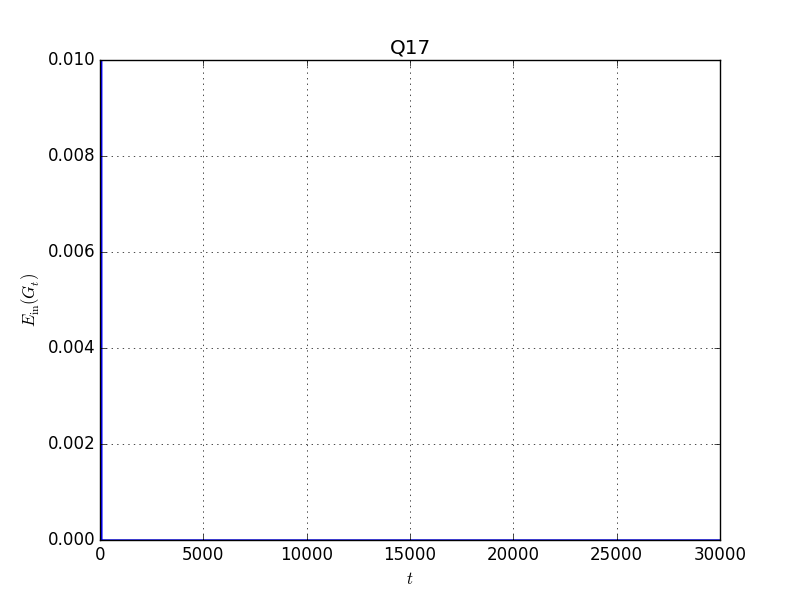
\includegraphics[scale=0.6]{Q17.png}
	\caption{Q17}
	\label{Q17}
\end{figure}
The average $E_{\text{in}}\ParTh{G_t}$ of total 30,000 trees is $0$. Since most values are 0 so the figure seems nothing left.
\begin{figure}[H]
	\centering
	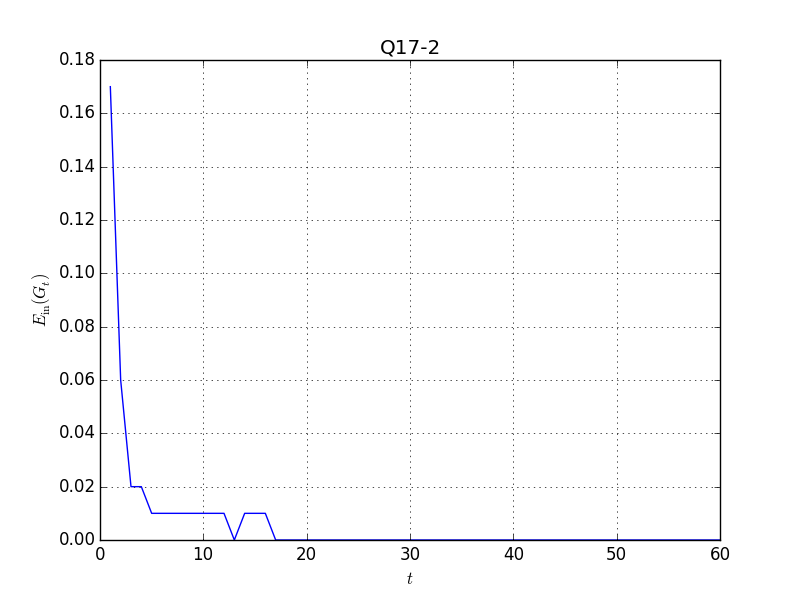
\includegraphics[scale=0.6]{Q17-2.png}
	\caption{Q17 first 60 points}
	\label{Q17-2}
\end{figure}
The figure of first 60 points. We can see that after the ${20}^{\text{th}}$ point, $E_{\text{in}}\ParTh{G_t}$ is almost 0.
\begin{figure}[H]
	\centering
	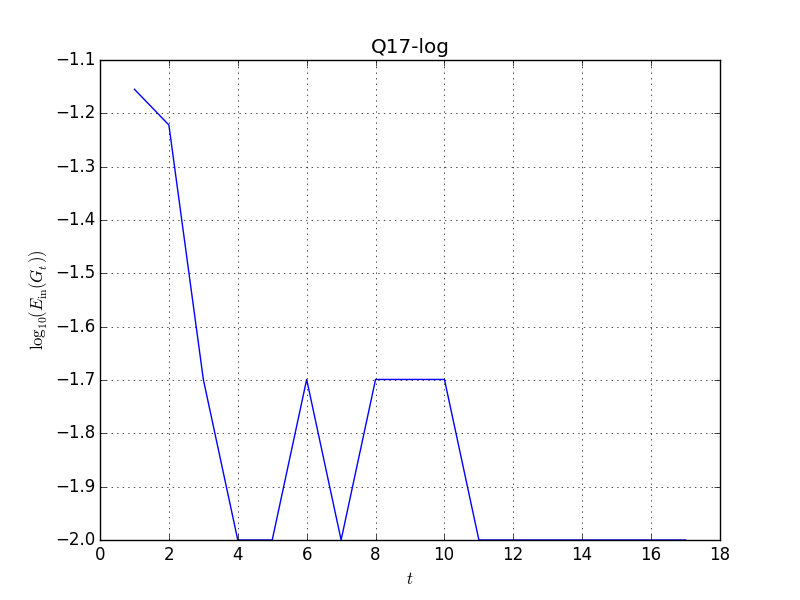
\includegraphics[scale=0.6]{Q17-log.png}
	\caption{Q17 $\log_{10}\ParTh{E_{\text{in}}\ParTh{G_t}}$}
	\label{Q17-log}
\end{figure}
The figure of log value of $E_{\text{in}}\ParTh{G_t}$ (removed $E_{\text{in}}\ParTh{G_t}=0$ points).

We can see that most of the $E_{\text{in}}\ParTh{G_t}=0$ (only 17 points left).

\QEDB

\horrule{0.5pt}

\subsection*{Problem 18}

\begin{figure}[H]
	\centering
	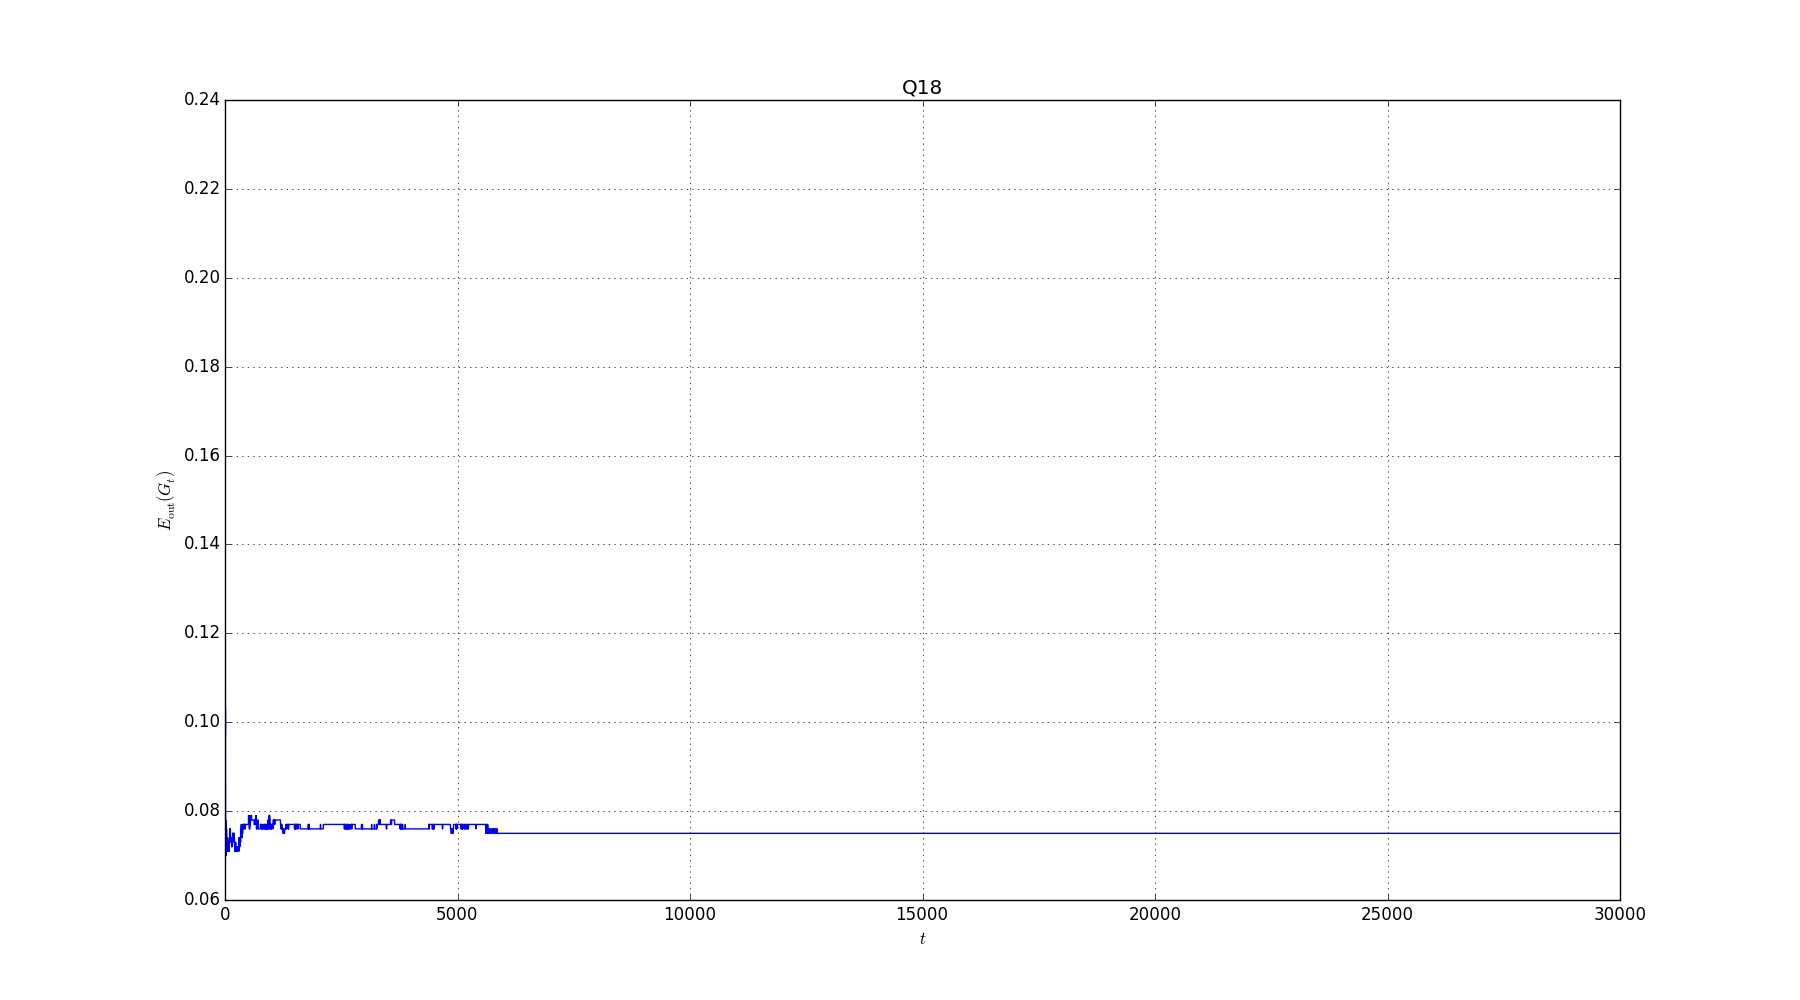
\includegraphics[scale=0.3]{Q18.png}
	\caption{Q18}
	\label{Q18}
\end{figure}
The average $E_{\text{out}}\ParTh{G_t}$ of total 30,000 trees is $0.0753$.

This curve approaches the average value as $t\rightarrow30,000$. The curve of Problem 17 goes to 0 after $t$ is near 20. Both curves converge to the average value as $t$ grows.

\QEDB

\horrule{0.5pt}

\subsection*{Problem 19}

\begin{figure}[H]
	\centering
	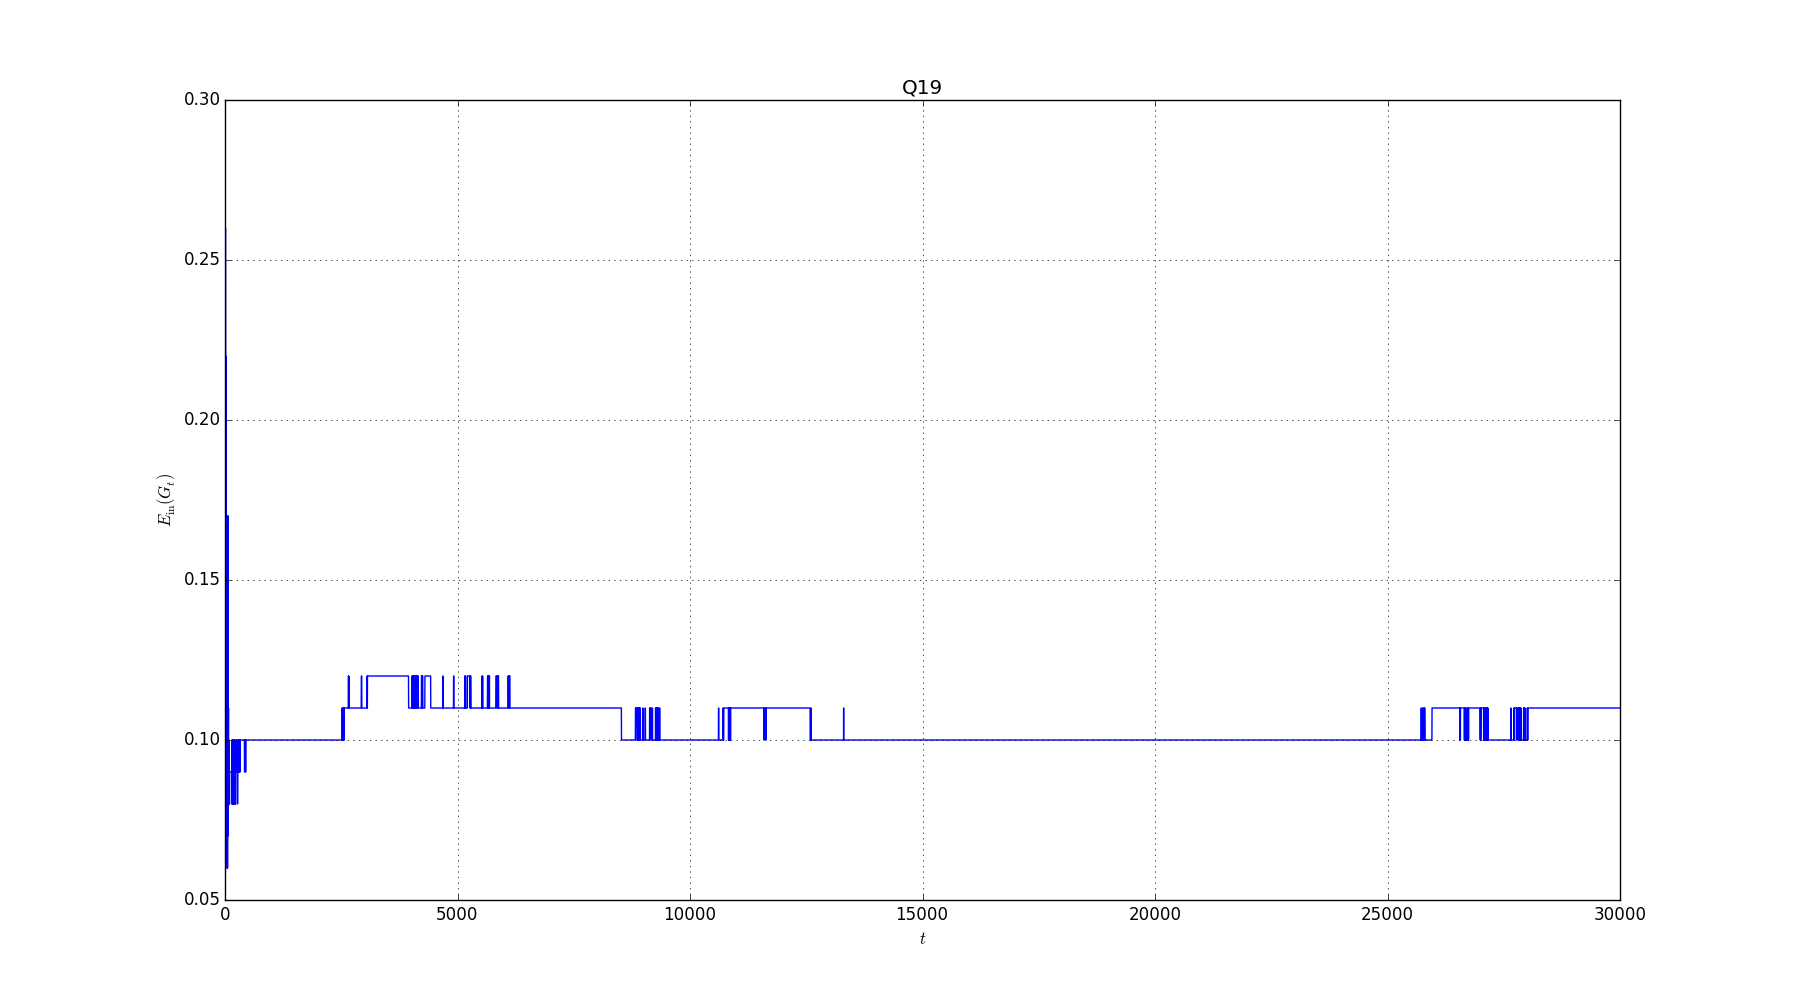
\includegraphics[scale=0.3]{Q19.png}
	\caption{Q19}
	\label{Q19}
\end{figure}
The average $E_{\text{in}}\ParTh{G_t}$ of total 30,000 trees is $0.1042$.

\QEDB

\horrule{0.5pt}

\subsection*{Problem 20}

\begin{figure}[H]
	\centering
	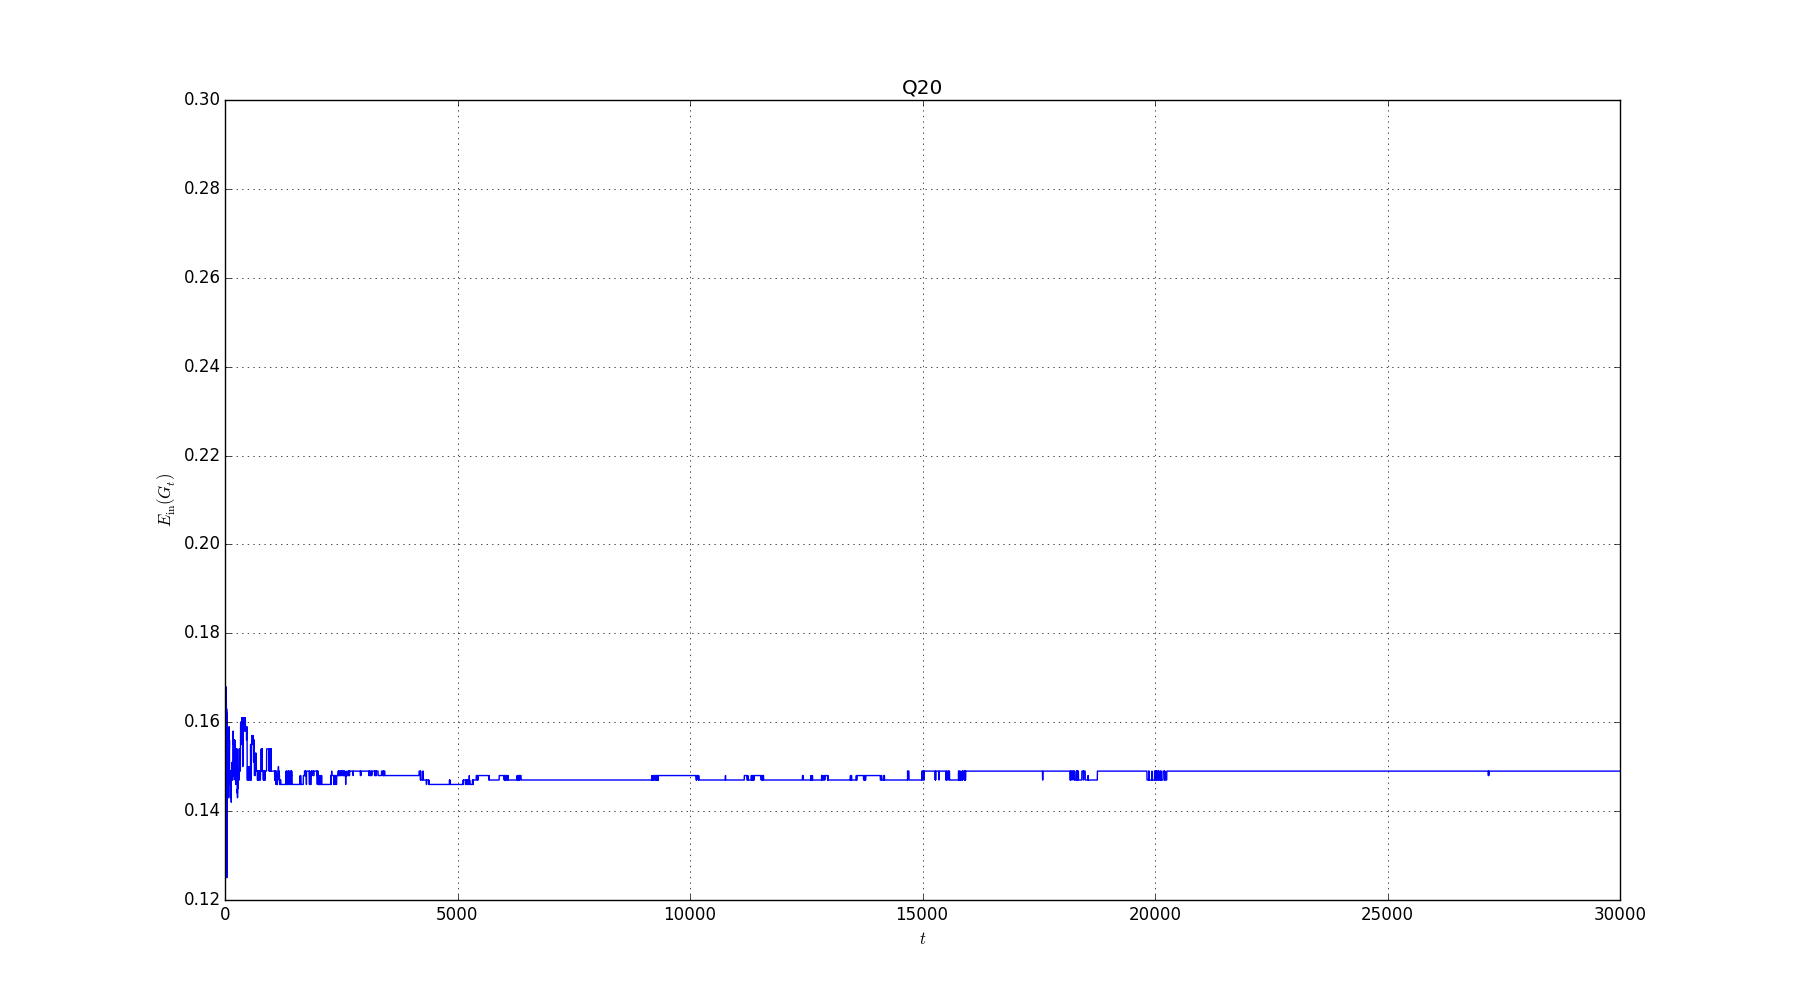
\includegraphics[scale=0.3]{Q20.png}
	\caption{Q20}
	\label{Q20}
\end{figure}
The average $E_{\text{out}}\ParTh{G_t}$ of total 30,000 trees is $0.1483$.

This curve approaches the average value as $t\rightarrow30,000$. The curve of Problem 19 oscillates between the average value.

\QEDB

\horrule{0.5pt}

\subsection*{Problem 21}

\begin{comment}
The weights of hidden layer and output layer are
\begin{align}
\text{Neuron 1}:\ParTh{w^{\ParTh{1}}_{01},w^{\ParTh{1}}_{11},w^{\ParTh{1}}_{21},\ldots,w^{\ParTh{1}}_{d1}}&=\ParTh{d-1,1,1,\ldots,1}\\
\text{Neuron 2}:\ParTh{w^{\ParTh{1}}_{02},w^{\ParTh{1}}_{12},w^{\ParTh{1}}_{22},\ldots,w^{\ParTh{1}}_{d2}}&=\ParTh{d-2,1,1,\ldots,1}\\
&\hspace{2mm}\vdots\\
\text{Neuron }d:\ParTh{w^{\ParTh{1}}_{0d},w^{\ParTh{1}}_{1d},w^{\ParTh{1}}_{2d},\ldots,w^{\ParTh{1}}_{dd}}&=\ParTh{0,1,1,\ldots,1}\\
\text{Output Neuron}:\ParTh{w^{\ParTh{2}}_{01},w^{\ParTh{2}}_{11},w^{\ParTh{2}}_{21},\ldots,w^{\ParTh{2}}_{d1}}&=\ParTh{0,1,-1,\ldots,\ParTh{-1}^{i-1},\ldots,1}
\end{align}
where $i\in\mathbb{N}$ and $1\leq i\leq d$.
\end{comment}
Map all possible inputs to $D$-dimension hypercube convex points. For example, $D=2$, all possible inputs are $\ParTh{-1,-1}$, $\ParTh{+1,-1}$, $\ParTh{-1,+1}$ and $\ParTh{+1,+1}$. Then we can construct a square lies on $x\text{-}y$ plane with convex points $\ParTh{-1,-1}$, $\ParTh{+1,-1}$, $\ParTh{-1,+1}$ and $\ParTh{+1,+1}$.

%Consider the projection of all convex points to diagonal line of $N$-dimensional hypercube, the value of each $\text{XOR}\ParTh{\text{convex point}}$ is
For a $N$-dimensional hypercube, the value of each $\text{XOR}\ParTh{\text{convex point}}$ is
\begin{enumerate}
	\item 2-D: $\ParTh{\text{XOR}\ParTh{-1,-1},\text{XOR}\ParTh{+1,-1},\text{XOR}\ParTh{-1,+1}\text{XOR}\ParTh{+1,+1}}=\ParTh{-1,+1,+1,-1}$
	\item 3-D: $\cdots=\ParTh{-1,+1,+1,+1,-1,-1,-1,+1}$
	%\item 4-D: $\cdots=\ParTh{-1,+1,+1,+1,+1,-1,-1,-1,-1,-1,-1,+1,+1,+1,+1,+1}$
	\item[$\vdots$]
\end{enumerate}
It is a little messy. Group the values by seperating $+1$ and $-1$, we have
\begin{enumerate}
	\item 2-D: $\underbrace{\ParTh{-1}}_{0\text{ input } +1},\underbrace{\ParTh{+1,+1}}_{1\text{ input } +1},\underbrace{\ParTh{-1}}_{2\text{ input } +1}$
	\item 3-D: $\underbrace{\ParTh{-1}}_{0\text{ input } +1},\underbrace{\ParTh{+1,+1,+1}}_{1\text{ input } +1},\underbrace{\ParTh{-1,-1,-1}}_{2\text{ input } +1},\underbrace{\ParTh{+1}}_{3\text{ input } +1}$
	%\item 4-D: $\ParTh{-1},\ParTh{+1,+1,+1,+1},\ParTh{-1,-1,-1,-1,-1,-1},\ParTh{+1,+1,+1,+1},\ParTh{+1}$
	\item[$\vdots$]
\end{enumerate}
We can see that $n$-dimension can be seperated to $\ParTh{n+1}$ groups, where $1\leq n\leq d$, $n\in\mathbb{N}$. Each group represents different output of $+1$ or $-1$. For example, $D=2$, $\text{XOR}\ParTh{-1,+1}=\text{XOR}\ParTh{+1,-1}=1$ so the two points (inputs) are in the same group. \\

Consider the orthogonal projection of of all convex points onto hyperline $x_1=x_2=\cdots=x_d$, we can find that the points in the same group will be projected onto the same point. For example, $D=2$, the projections of $\ParTh{-1,+1}$ and $\ParTh{+1,-1}$ onto $y=x$ are both $\ParTh{0,0}$. This can be proved by calculating the shortest distance to the hyperline for all points with same number of $+1$ inputs,
\begin{align}
\text{Shortest Distance}=\sum_{i=1}^{k}\ParTh{x_i-1}^2+\sum_{j=1}^{d-k}\ParTh{x_j+1}^2=d\ParTh{x-1}^2+\ParTh{d-k}\ParTh{x+1}^2
\end{align}
where $k$ is the number of $+1$ of some input and set $x_1=x_2=\cdots=x_d=x$. So the projections of all points with same number of $+1$ inputs onto the hyperline is the same point.\\
%; $D=3$, the projections of $\ParTh{-1,-1,+1}$, $\ParTh{-1,+1,-1}$ and $\ParTh{+1,-1,-1}$ onto $x+y+z+1=0$ are all $\ParTh{0,0}$.

The $d\text{-}D\text{-}1$ neural network is trying to classify all these inputs into different groups. One neuron in the hidden layer with $\ParTh{d+1}$ weights $\ParTh{w^{\ParTh{\ell}}_{0j},w^{\ParTh{\ell}}_{1j},\ldots,w^{\ParTh{\ell}}_{dj}}$ can only construct a hyperplane in $d$-dimension (since one weight is from constant input), like a classfier, seperating the convex points of hypercube into different group. And $d$-dimension hypercube needs at least $d$ hyperplanes to seperate all convex points (inputs) into $\ParTh{d+1}$ groups (output).

For example, $D=2$, then we have three points $\ParTh{-1,-1}$, $\ParTh{0,0}$ and $\ParTh{+1,+1}$ after projection. We can find the hyperplane $x+y=1$ and $-x-y=1$ with corresponding neurons of $\ParTh{+1,+1,+1}$ and $\ParTh{+1,-1,-1}$ in hidden layer, neuron of $\ParTh{-1,+1,+1}$ in output layer. These hyperplanes can seperate all convex points into three groups. So we can implement $\text{XOR}\ParTh{x_1,x_2}$. Similarly, we can implement $\text{XOR}\ParTh{x_1,x_2,\ldots,x_d}$.

Hence, we need at least $D=d$ to implement $\text{XOR}\ParTh{x_1,x_2,\ldots,x_d}$ with $d\text{-}D\text{-}1$ feed-forward neural network.

\QEDB

\horrule{0.5pt}

\subsection*{Problem 22}

\underline{Claim}: If $d$ is odd, then $D\geq \ParTh{\Divide{\ParTh{d+1}}{2}}$; if $d$ is even, then we have $D\geq \ParTh{\Divide{d}{2}}+1$. Two cases can be implemented by $d\text{-}\ParTh{D-1}\text{-}1$ feed-forward neuron network.

\underline{Proof of Claim}:

From the groups seperated in Problem 21, we can find that they are symmetric. If we can connect all inputs directly to output neuron, we can specify which side are we on by $\text{ADD}$ all inputs to see if $\sum_{i=1}^{d}x_i\lessgtr0$ (for $d$ is odd) or $\sum_{i=1}^{d}x_i\lesseqgtr0$ (for $d$ is even).

For example, $D=2$, we have
\begin{align}
\left.\underbrace{\ParTh{-1}}_{0\text{ input } +1}\middle|\underbrace{\ParTh{+1,+1}}_{1\text{ input } +1}\middle|\underbrace{\ParTh{-1}}_{2\text{ input } +1}\right.\Rightarrow\left.\underbrace{\ParTh{+1,+1}}_{\text{ Inputs summation is }0}\middle|\underbrace{\ParTh{-1}}_{\text{ Inputs summation is }\lessgtr\text{ 0}}\right.
\end{align}
or $D=3$,
\begin{align}
\left.{\ParTh{-1}}\Big\vert{\ParTh{+1,+1,+1}}\Big\vert{\ParTh{-1,-1,-1}}\Big\vert{\ParTh{+1}}\right.&\Rightarrow\underbrace{\left.{\ParTh{-1,-1,-1}}\Big\vert{\ParTh{+1}}\right.}_{\text{ Inputs summation }>\text{ 0}}\\
\nonumber
&\text{or }\underbrace{\left.{\ParTh{+1,+1,+1}}\Big\vert{\ParTh{-1}}\right.}_{\text{ Inputs summation }<\text{ 0}}
\end{align}

Hence we can reduce the number of neurons in hidden layer by half, which is $\Divide{\ParTh{d-1}}{2}$ for $d$ is odd and $\ParTh{\Divide{d}{2}}$ for $d$ is even, where $\Divide{\ParTh{d-1}}{2}$ is due to we do not need the central hyperplane to seperate the inputs.

Plus the neuron in output layer, we have $D\geq \ParTh{\Divide{\ParTh{d+1}}{2}}$ if $d$ is odd and $D\geq \ParTh{\Divide{d}{2}}+1$ if $d$ is even.

\begin{comment}
\begin{enumerate}
\item $d$ is even.

From the conclusion of Problem 21, we need at least $D=d+1$ ($d$ for hidden layer and $1$ for output layer). But now we can connect all inputs directly to output neuron to distinguish $\ParTh{-1,-1,\ldots,-1}$ and $\ParTh{+1,+1,\ldots,+1}$ with weights $\ParTh{0,+1,+1,\ldots,+1}$. Hence we can use one less neuron.
\item $d$ is odd.

If $d$ is odd, from the conclusion of Problem 21, we need $d$ hyperplanes to seperate all inputs, where $d$ is odd. So all inputs 
\end{enumerate}

The answer is $D=d-1$. Like
\begin{figure}[H]
	\centering
	\begin{tikzpicture}[auto]
	% Node Setting %
	\node [point] (x0) {$x_0=+1$};
	\node [point, below of = x0] (x1) {$x_1$};
	\node [point, below of = x1] (x2) {$x_2$};
	\node [point, below of = x2] (xdots) {$\vdots$};
	\node [point, below of = xdots] (xd_1) {$x_{d-1}$};
	\node [point, below of = xd_1] (xd) {$x_d$};
	\node [cloud, right of = x0, xshift=1.5cm] (n0) {$\scriptstyle+1$};
	\node [cloud, right of = x1, xshift=1.5cm] (n1) {$1$};
	%\node [cloud, right of = x2, xshift=1.5cm] (n2) {$2$};
	\node [point, right of = xdots, xshift=1.5cm, yshift=0.5cm] (ndots) {$\vdots$};
	\node [cloud, right of = xd_1, xshift=1.5cm, yshift=-0.7cm] (nd) {$\scriptstyle{d-2}$};
	\node [cloud, above right of = ndots, xshift=1.5cm] (out) {$\scriptstyle{d-1}$};
	% Connection %
	\path [line] (x0)  -- (n1);
	\path [line] (x1)  -- (n1);
	\path [line] (x2)  -- (n1);
	\path [line] (xd_1)  -- (n1);
	\path [line] (xd)  -- (n1);
	%\path [line] (x0)  -- (n2);
	%\path [line] (x1)  -- (n2);
	%\path [line] (x2)  -- (n2);
	%\path [line] (xd_1)  -- (n2);
	%\path [line] (xd)  -- (n2);
	\path [line] (x0)  -- (nd);
	\path [line] (x1)  -- (nd);
	\path [line] (x2)  -- (nd);
	\path [line] (xd_1)  -- (nd);
	\path [line] (xd)  -- (nd);
	\path [line] (n0)  -- (out);
	\path [line] (n1)  -- (out);
	%\path [line] (n2)  -- (out);
	\path [line] (nd)  -- (out);
	\path [line] (x1)  -- (out);
	\path [line] (x2)  -- (out);
	\path [line] (xd_1)  -- (out);
	\path [line] (xd)  -- (out);
	\end{tikzpicture}
	\label{LTC}
\end{figure}
\end{comment}

\QEDB

\horrule{0.5pt}

\section*{Reference}

\begin{enumerate}

\item[{[1]}] Lecture Notes by Hsuan-Tien LIN, Department of Computer Science and Information Engineering, National Taiwan University, Taipei 106, Taiwan.

\end{enumerate}

\end{document}